%\documentclass[12pt,serif]{beamer}
%\documentclass[tikz,12pt,svgnames]{beamer}
\documentclass[table,handout,tikz,12pt,svgnames]{beamer}
\usepackage{CM-preamble}
\subtitle{\LARGE Les Arbres}
\date{CM7}

%README TODO STUFF

\begin{document}

\begin{frame}
	\titlepage
\end{frame}

\begin{frame}[fragile=singleslide]
	\frametitle{Les arbres}
		\begin{block}{Collection d'informations hiérarchisées}
		\end{block}
		\begin{block}{Exemple}
			\begin{itemize}
				\item Arbre généalogique, organigramme d'une entreprise, table des matières d'un livre
				\item Organisation d'informations dans une base de données, représentation de la structure syntaxique d'un programme dans les compilateurs
			\end{itemize}
		\end{block}
%		\IMAGE
\end{frame}


\begin{frame}[fragile=singleslide]
	\frametitle{Les arbres: terminologie}
	\vspace{-4em}
	\begin{block}{}
    \begin{adjustwidth}{-0.9cm}{}
		
		\begin{center}
		{\includegraphics[scale=0.58]{../common-images/arbre.pdf}}
		\end{center}
	\end{adjustwidth}
	\end{block}
\end{frame}


\begin{frame}[fragile=singleslide]
	\frametitle{Les arbres: définitions}
	\begin{block}{}
		\begin{itemize}
			\item \underline{\textbf{Niveau d'un nœud}} : nombre d'arêtes entre le nœud et la racine (ex : niveau de s3.2 = 2)
			\item \underline{\textbf{Hauteur d'un arbre}} : niveau maximum de l'arbre (3 pour l'exemple)
			\item \underline{\textbf{Arbre ordonné}} : l'ordre des fils de chaque nœud est spécifié
			\item \underline{\textbf{Degré d'un nœud}} : nombre de fils que le nœud possède
			\item \underline{\textbf{Arbre n-aire}} : les nœuds sont de degré n
		\end{itemize}
	\end{block}
\end{frame}


\begin{frame}[fragile=singleslide]
	\frametitle{Les arbres binaires}
	\vspace{1cm}
	\begin{block}{Définition}
		\vspace{0.5em}		
		\texttt{B = $\emptyset$ | < R, G, D >}
%	\begin{itemize}
%		\item 
%		\mintinline{c}{FILE *fopen (char *nom, char *mode)} où
		\vspace{0.5em}
		\small
		\[
		\hspace{-5cm}
		\texttt{où} 
		\begin{cases}
		\texttt{R}: & \text{Noeud Racine}\\
		\texttt{G}: & \text{Sous-arbre gauche}\\
		\texttt{D}: & \text{Sous-arbre droite}\\
%		\texttt{rb+}: & \text{lecture/écriture}	\\\ldots
		\end{cases}
		\]
		\vspace{-1em}
%	\end{itemize}
	\end{block}
	\vspace{1cm}
	\begin{block}{Exemple}
%		\IMAGE
		\vspace{-2.5cm}
		\begin{flushright}
			{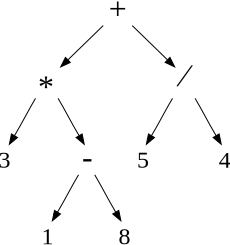
\includegraphics[scale=0.5]{../common-images/arbre2.pdf}}
		\end{flushright}
	\end{block}
\end{frame}


\begin{frame}[fragile=singleslide]
	\frametitle{Le \textit{type} arbre binaire}
	\vspace{-1em}
	\begin{block}{} %Déclaration}
		\begin{itemize}
			\item \textbf{Déclaration :} \texttt{A \underline{de type} ArbreBinaire \underline{de} <T>}
		\end{itemize}
	\end{block}
	\begin{block}{Primitives}
		\begin{itemize}%[leftmargin=1ex]
			\item \texttt{init\_arbre(A)} : crée un arbre binaire vide
			\item \texttt{vide(A)} : teste si \texttt{A} vide
			\item \texttt{valeur(A)} : retourne la valeur de la racine
			\item \texttt{gauche(A)} : retourne le sous-arbre gauche de \texttt{A}
			\item \texttt{droite(A)} : retourne le sous-arbre droit
			\item \texttt{put\_valeur(A,V)} : range la valeur de \texttt{V} à la racine
			\item \texttt{put\_droite(A,D)} : \texttt{D} devient le sous-­arbre droit de \texttt{A}
			\item \texttt{put\_gauche(A,G)} : \texttt{G} devient le sous-arbre gauche de \texttt{A} 
			\item \texttt{cons(R, G, D)} : construit l'arbre \texttt{<R, G, D>}
		\end{itemize}
	\end{block}
\end{frame}


\begin{frame}[fragile=singleslide]
	\frametitle{Le \textit{type} arbre binaire: exemple}
%	\vspace{-1em}
	\begin{block}{} %Déclaration}
		\begin{itemize}
			\item Fonction qui teste si un arbre est une feuille\\(1 seul nœud)			
		\end{itemize}
	\end{block}
	\begin{block}{}
		\begin{minted}[mathescape=true,escapeinside=||,tabsize=4,fontsize=\footnotesize,]{c}
	|\underline{Fonction}| feuille(A)
		|\underline{D}| : A : ArbreBinaire |\underline{de}| <T>
		|\underline{Si}| vide(A) |\underline{Alors}|
			retourner (faux)
		|\underline{Sinon}|
			retourner( vide(gauche(A)) et vide(droite(A)) )
		|\underline{Fsi}|
	|\underline{Ffonction}|		
		\end{minted}		
	\end{block}
\end{frame}

\begin{frame}[fragile=singleslide]
	\frametitle{Le \textit{type} arbre binaire: exemple}
	%	\vspace{-1em}
	\begin{block}{} %Déclaration}
		\begin{itemize}
			\item Calcul du nombre de noeuds d'un arbre binaire
		\end{itemize}
	\end{block}

	\begin{block}{}%Définition}
%		\vspace{0.5em}		
%		\texttt{B = $\emptyset$ | < R, G, D >}
		%	\begin{itemize}
		%		\item 
		%		\mintinline{c}{FILE *fopen (char *nom, char *mode)} où
		\vspace{-1.5em}
		\small
		\[
		\hspace{-0.5cm}
		\texttt{nb\_noeuds(A)} 
		\begin{cases}
		\texttt{A = $\emptyset$}: & \texttt{0}\\
		\texttt{A = <R,G,D>}: & \texttt{1} + \texttt{nb\_noeuds(G)} + \texttt{nb\_noeuds(D)}
		
		%		\texttt{rb+}: & \text{lecture/écriture}	\\\ldots
		\end{cases}
		\]
		\vspace{-1em}
		%	\end{itemize}
	\end{block}

	\begin{block}{}
		\begin{minted}[mathescape=true,escapeinside=||,tabsize=4,fontsize=\footnotesize,]{c}
	|\underline{Fonction}| nb_noeuds(A)
		|\underline{D}| : A : ArbreBinaire |\underline{de}| <T>
		|\underline{Si}| vide(A) |\underline{Alors}|
			retourner (0)
		|\underline{Sinon}|
			retourner ( 1 + nb_noeuds(G) + nb_noeuds(D) )
		|\underline{Fsi}|
	|\underline{Ffonction}|		
		\end{minted}		
	\end{block}
\end{frame}


\begin{frame}[fragile=singleslide]
	\frametitle{Algorithmes sur les arbres}
	\begin{block}{3 types de parcours pour effectuer un traitement sur tous les noeuds}
		\begin{itemize}
			\item Préfixé
			\item Postfixé
			\item Infixé
		\end{itemize}
	\end{block}
\end{frame}

\begin{frame}[fragile=singleslide]
	\frametitle{Les arbres: parcours prefixé ou \texttt{RGD}}
	\begin{block}{Parcours prefixé ou \texttt{RGD}}
		\begin{itemize}
			\item Traiter la racine
			\item Traiter le sous-arbre gauche
			\item Traiter le sous-arbre droit
		\end{itemize}
	\end{block}
\end{frame}


\begin{frame}[fragile=singleslide]
	\frametitle{Les arbres: parcours prefixé ou \texttt{RGD}}
	\begin{block}{}
%		\begin{minted}[mathescape=true,escapeinside=||,tabsize=4,fontsize=\footnotesize,]{c}
%|\underline{Action}| RGD(A)
%	|\underline{D}| : A : ArbreBinaire |\underline{de}| <T>
%	|\underline{Si}| non vide(A) |\underline{Alors}|
%		traiter(valeur(A))
%		RGD(gauche(A))
%		RGD(droite(A))
%	|\underline{Fsi}|
%|\underline{Faction}|		
%		\end{minted}
		\begin{columns}[T]
%			\hspace{-0.5cm}
			\begin{column}{0.7\textwidth}
				\begin{minted}[mathescape=true,escapeinside=||,tabsize=4,
				%fontsize=\footnotesize,
				]{c}
|\underline{Action}| RGD(A)
	|\underline{D}| : A : ArbreBinaire |\underline{de}| <T>
	|\underline{Si}| non vide(A) |\underline{Alors}|
		traiter(valeur(A))
		RGD(gauche(A))
		RGD(droite(A))
	|\underline{Fsi}|
|\underline{Faction}|
		
				\end{minted}
			\end{column}
			%		\setlength{\columnseprule}{0.4pt}
			\hspace{-2.5cm}
%			\vrule{}
			\hspace{0.2cm}
			\begin{column}{0.38\textwidth}
				\begin{flushright}
					{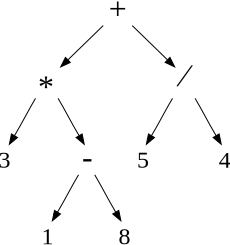
\includegraphics[scale=0.45]{../common-images/arbre2.pdf}}
				\end{flushright}
			\end{column}
		\end{columns}
		\vspace{0.5cm}
		Exemple :\\ \texttt{traiter(valeur(A)) = écrire(valeur(A))}\\
		$\Rightarrow$ \texttt{+ * 3 - 1 8 / 5 4} (notation préfixée)
	\end{block}
%	\IMAGE
\end{frame}


\begin{frame}[fragile=singleslide]
	\frametitle{Les arbres: parcours postfixé ou \texttt{GDR}}
	\begin{block}{Parcours postfixé ou \texttt{GDR}}
		\begin{itemize}
			\item Traiter le sous-arbre gauche
			\item Traiter le sous-arbre droit
			\item Traiter la racine
		\end{itemize}
	\end{block}
\end{frame}


\begin{frame}[fragile=singleslide]
	\frametitle{Les arbres: parcours postfixé ou \texttt{GDR}}
	\begin{block}{}
		\begin{columns}[T]
			\begin{column}{0.7\textwidth}
				\begin{minted}[mathescape=true,escapeinside=||,tabsize=4,
				%fontsize=\footnotesize,
				]{c}
|\underline{Action}| GDR(A)
	|\underline{D}| : A : ArbreBinaire |\underline{de}| <T>
	|\underline{Si}| non vide(A) |\underline{Alors}|
		GDR(gauche(A))
		GDR(droite(A))
		traiter(valeur(A))
	|\underline{Fsi}|
|\underline{Faction}|		
				\end{minted}
			\end{column}
			%		\setlength{\columnseprule}{0.4pt}
			\hspace{-2.5cm}
			%			\vrule{}
			\hspace{0.2cm}
			\begin{column}{0.38\textwidth}
				\begin{flushright}
					{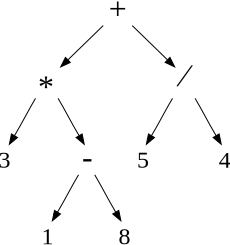
\includegraphics[scale=0.45]{../common-images/arbre2.pdf}}
				\end{flushright}
			\end{column}
		\end{columns}
		\vspace{0.5cm}		
		Exemple :\\ \texttt{traiter(valeur(A)) = écrire(valeur(A))}\\
		$\Rightarrow$ \texttt{3 1 8 - * 5 4 / +} (notation postfixée)
	\end{block}
%	\IMAGE
\end{frame}


\begin{frame}[fragile=singleslide]
	\frametitle{Les arbres: parcours infixé ou \texttt{GRD}}
	\begin{block}{}%Parcours postfixé ou \texttt{GRD}}
		\begin{itemize}
			\item Traiter le sous-arbre gauche
			\item Traiter la racine
			\item Traiter le sous-arbre droit
		\end{itemize}
	\end{block}
	\begin{block}{}
		\begin{minted}[mathescape=true,escapeinside=||,tabsize=4,
		%fontsize=\footnotesize,
		]{c}
	|\underline{Action}| GRD(A)
		|\underline{D}| : A : ArbreBinaire |\underline{de}| <T>
		|\underline{Si}| non vide(A) |\underline{Alors}|
			GRD(gauche(A))
			traiter(valeur(A))
			GRD(droite(A))
		|\underline{Fsi}|
	|\underline{Faction}|		
		\end{minted}
%		Exemple : \texttt{traiter(valeur(A)) = écrire(valeur(A))}\\
%		$\Rightarrow$ \texttt{3 1 8 - * 5 4 / +} (notation postfixée)
	\end{block}
%	\IMAGE
\end{frame}

\begin{frame}[fragile=singleslide]
	\frametitle{Implantation des arbres binaires}
	\begin{block}{Représentation par pointeurs}%Parcours postfixé ou \texttt{GRD}}
		\begin{center}
			{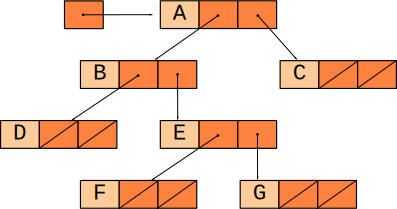
\includegraphics[scale=0.9]{../common-images/arbre3.pdf}}
		\end{center}
	\end{block}
\end{frame}


\begin{frame}[fragile=singleslide]
	\frametitle{Implantation des arbres binaires}
	\begin{minted}[mathescape=true,escapeinside=||,tabsize=4
%		,fontsize=\footnotesize,
		]{c}
	|\underline{type}| ArbreBinaire = pointeur |\underline{de}| Noeud

	|\underline{type}| Noeud = |\underline{structure}|
			val : <T>
			gauche, droit: ArbreBinaire
	|\underline{fin}|
	\end{minted}
%	\begin{block}{Soit \texttt{A} un \texttt{ArbreBinaire}}%Représentation par pointeurs}%Parcours postfixé ou \texttt{GRD}}
%%		\begin{itemize}
%%			\item \texttt{vide(A)      |$\Rightarrow$| retourner(A = NULL)}
%%			\item \texttt{initArbre(A) |$\Rightarrow$| A $\leftarrow$ NULL}
%%			\item \texttt{valeur(A)    |$\Rightarrow$| retourner(A$\uparrow$$\bullet$val)}
%%			\item \texttt{gauche(A)    |$\Rightarrow$| retourner(A$\uparrow$$\bullet$gauche)}
%		\begin{minted}[mathescape=true,escapeinside=||,tabsize=4,fontsize=\footnotesize,]{c}
%	vide(A)       |$\Rightarrow$|   retourner(A = NULL)
%	init_arbre(A) |$\Rightarrow$|   A |$\leftarrow$| NULL
%	valeur(A)     |$\Rightarrow$|   retourner(A|$\uparrow$$\bullet$|val)
%	gauche(A)     |$\Rightarrow$|   retourner(A|$\uparrow$$\bullet$|gauche)
%		\end{minted}
%			
%%		\end{itemize}
%	\end{block}
\end{frame}


\begin{frame}[fragile=singleslide]
	\frametitle{Implantation des arbres binaires}
	\begin{block}{Soit \texttt{A} un \texttt{ArbreBinaire}}
		\begin{minted}[mathescape=true,escapeinside=||,tabsize=4,fontsize=\footnotesize,]{c}
	vide(A)         |$\Rightarrow$|   retourner(A = NULL)
	init_arbre(A)   |$\Rightarrow$|   A |$\leftarrow$| NULL
	valeur(A)       |$\Rightarrow$|   retourner(A|$\uparrow$$\bullet$|val)
	gauche(A)       |$\Rightarrow$|   retourner(A|$\uparrow$$\bullet$|gauche)
	droite(A)       |$\Rightarrow$|   retourner(A|$\uparrow$$\bullet$|droite)
	put_valeur(A,V) |$\Rightarrow$|   A|$\uparrow$$\bullet$|val    |$\leftarrow$| V
	put_gauche(A,G) |$\Rightarrow$|   A|$\uparrow$$\bullet$|gauche |$\leftarrow$| G
	put_droite(A,D) |$\Rightarrow$|   A|$\uparrow$$\bullet$|droit  |$\leftarrow$| D

	cons(V,G,D)     |$\Rightarrow$|   allouer(A)
                         A|$\uparrow$$\bullet$|val    |$\leftarrow$| V
                         A|$\uparrow$$\bullet$|gauche |$\leftarrow$| G
                         A|$\uparrow$$\bullet$|droit  |$\leftarrow$| D
	
	
		\end{minted}
%	cons(R,G,D)     |$\Rightarrow$|   allouer(A)		
%		TODO: VERIFY CONS(), MAYBE IT'S BETTER IF IT'S V AND NOT R
		%		\end{itemize}
	\end{block}
\end{frame}


\begin{frame}[fragile=singleslide]
	\frametitle{Les arbres binaires ordonnées}
	\begin{block}{Rappel}
		\begin{itemize}
			\item Liste contiguë : recherche dichotomique en $O(log_2n)$\\
			Ajout / suppression en $O(n)$ 
			\item Liste chaînée : recherche en $O(n)$\\
			Ajout / suppression en temps constant
		\end{itemize}
	\end{block}
	\begin{block}{Arbre binaire ordonné (ou arbre de recherche)}
		\begin{itemize}
			\item Recherche / ajout / suppression : même efficacité
			\item Au mieux (arbre équilibré) en $log_2(n)$
		\end{itemize}
	\end{block}
\end{frame}


\begin{frame}[fragile=singleslide]
	\frametitle{Les arbres binaires ordonnées: définition}
	\begin{block}{Soit \texttt{A = <R, G, D>}, \texttt{A} est ordonné si}
		\begin{itemize}
			\item Pour tout nœud \texttt{nd} de \texttt{G}, \texttt{valeur(nd)} $\leq$ \texttt{R}
			\item Pour tout nœud \texttt{nd} de \texttt{D}, \texttt{valeur(nd)} $>$ \texttt{R}
			\item \texttt{G} et \texttt{D} sont des arbres ordonnés
		\end{itemize}
	\end{block}
	\begin{center}
		{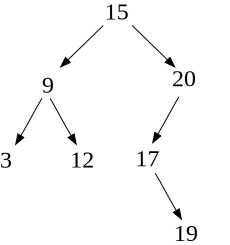
\includegraphics[scale=0.4]{../common-images/arbre4.pdf}}
	\end{center}
	\vspace{-1.1cm}
	\begin{block}{}
		\begin{itemize}
			\item Parcours \texttt{GRD} d'un arbre ordonné $\Rightarrow$ par ordre croissant
			\item Parcours \texttt{DRG} d'un arbre ordonné $\Rightarrow$ par ordre décroissant
		\end{itemize}
	\end{block}
\end{frame}


\begin{frame}[fragile=singleslide]
	\frametitle{Recherche dans un arbre binaire ordonné}
	\begin{block}{Recherche associative d'un élément \texttt{V}}
		\begin{itemize}
			\item \texttt{A} = $\emptyset$ $\Rightarrow$ non trouvé
			\item \texttt{A = <R, G, D>}
			\begin{itemize}
				\item \texttt{R = X $\Rightarrow$} trouvé
				\item \texttt{X < R $\Rightarrow$} rechercher \texttt{X} dans \texttt{G}
				\item \texttt{X > R $\Rightarrow$} rechercher \texttt{X} dans \texttt{D}	
			\end{itemize}
		\end{itemize}
	\end{block}
	\begin{block}{Coût de la recherche}
		\begin{itemize}
			\item Dans tous les cas $\leq$n
			\item Au mieux $log_2(n)$ si l'arbre est équilibré $\Rightarrow$ techniques de construction d'arbres équilibrés
		\end{itemize}
	\end{block}
\end{frame}


\begin{frame}[fragile=singleslide]
	\frametitle{Recherche dans un arbre binaire ordonné}
%	\begin{block}{}
	\vspace{-0.1cm}
	\begin{minted}[mathescape=true,escapeinside=||,tabsize=4
	%,fontsize=\footnotesize,
	]{c}
|\underline{Fonction}| existe(X, A) : booléen
	|\underline{D}| : X : <T> ; 
		A : ArbreBinaire
	|\underline{Si}| vide(A) |\underline{Alors}|
		retourner(faux)
	|\underline{Sinon}|
		|\underline{Si}| X=valeur(A) |\underline{Alors}|
			retourner(vrai)
		|\underline{Sinon}|
			|\underline{Si}| X < valeur(A) |\underline{Alors}| 
				retourner(existe(X,gauche(A)))
			|\underline{Sinon}|
				retourner(existe(X,droite(A)))
			|\underline{Fsi}|
		|\underline{Fsi}|
	|\underline{Fsi}|		
|\underline{Ffonction}|
		\end{minted}
		%	cons(R,G,D)     |$\Rightarrow$|   allouer(A)		
		%		TODO: VERIFY CONS(), MAYBE IT'S BETTER IF IT'S V AND NOT R
		%		\end{itemize}
%	\end{block}
\end{frame}


\begin{frame}[fragile=singleslide]
	\frametitle{Ajout dans un arbre binaire ordonné}
	\vspace{0.5cm}
	\begin{block}{Solution simple : ajout en feuille}
	\end{block}
	\begin{block}{}
		\vspace{-1.2cm}
		\begin{center}
			{\includegraphics[scale=0.65]{../common-images/arbre5.pdf}}
		\end{center}
	\end{block}
\end{frame}


\begin{frame}[fragile=singleslide]
	\frametitle{Ajout dans un arbre binaire ordonné}
	\begin{block}{\texttt{Ajout(A,V)} :}
		\begin{itemize}
			\item \texttt{A} = $\emptyset$ $\Rightarrow$ \texttt{A=<V,$\emptyset$,$\emptyset$>}
			\item \texttt{A = <R, G, D>}
			\begin{itemize}
				\item \texttt{V $\leq$ R $\Rightarrow$} ajouter \texttt{V} dans \texttt{gauche(A)}
				\item \texttt{V > R $\Rightarrow$} ajouter \texttt{V} dans \texttt{droite(A)}
			\end{itemize}
			\item Utilisation du passage de \texttt{A} en \texttt{D/R} pour établir le lien père/fils
			\item cf : algorithme récursif d'ajout d'un élément dans une liste chaînée			
		\end{itemize}
	\end{block}
\end{frame}


\begin{frame}[fragile=singleslide]
	\frametitle{Ajout dans un arbre binaire ordonné}
	%	\begin{block}{}
	\vspace{-0.1cm}
	\begin{minted}[mathescape=true,escapeinside=||,tabsize=4
	%,fontsize=\footnotesize,
	]{c}
|\underline{Action}| ajout(V, A)
	|\underline{D}| : V : <T> ; 
	|\underline{\textbf{D/R}}| : A : ArbreBinaire de <T>
	|\underline{Si}| vide(A) |\underline{Alors}|
		A |$\leftarrow$| cons(V,|$\emptyset$|,|$\emptyset$|)
	|\underline{Sinon}|
		|\underline{Si}| V |$\leq$| valeur(A) |\underline{Alors}|
			ajout (V, |\textbf{gauche(A)}|)
		|\underline{Sinon}|
			ajout (V, |\textbf{droite(A)}|)
		|\underline{Fsi}|
	|\underline{Fsi}|
|\underline{Faction}|
	\end{minted}
	%	cons(R,G,D)     |$\Rightarrow$|   allouer(A)		
	%		TODO: VERIFY CONS(), MAYBE IT'S BETTER IF IT'S V AND NOT R
	%		\end{itemize}
	%	\end{block}
\end{frame}
% % % % % % % % % % % % % % % % % % % % % % % % % % %
% END
% % % % % % % % % % % % % % % % % % % % % % % % % % %
\end{document}
% % % % % % % % % % % % % % % % % % % % % % % % % % %
% END
% % % % % % % % % % % % % % % % % % % % % % % % % % %